\section{Desktop Environment and Design Language}
\label{sec:desktop}

The desktop environment is the most visible part of the system and the primary
differentiator for users switching from other platforms. The goal is a fast,
coherent desktop that does not feel like a collection of independent projects
assembled by different teams in different decades. The stack reflects this:
performance-critical and system-close code is Rust, everything visual is
TypeScript with Tailwind CSS, and the two halves communicate over well-defined
interfaces that neither side reaches past.

\subsection{Architecture and IPC}
\label{sec:desktop-ipc}

Three communication channels connect the compositor core to the shell and its
frontend, each carrying a different class of data.

\begin{figure}[htbp]
\centering
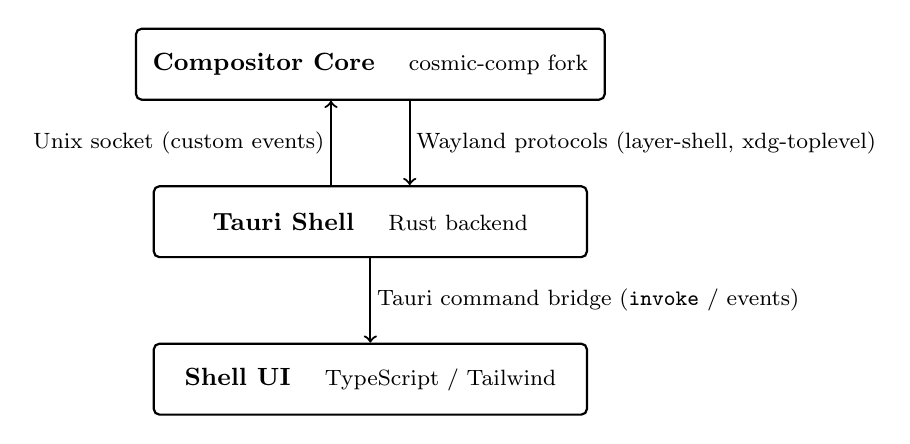
\begin{tikzpicture}[
	box/.style={
		draw, thick, rectangle, rounded corners=2pt,
		minimum width=5.5cm, minimum height=0.9cm,
		font=\small, align=center, inner sep=6pt
	},
	arr/.style={->, thick},
	lbl/.style={font=\footnotesize, fill=white, inner sep=2pt, align=center},
	]
	
	\node[box] (smithay) at (0, 4.0) {\textbf{Compositor Core} \quad {\footnotesize cosmic-comp fork}};
	\node[box] (tauri)   at (0, 2.0) {\textbf{Tauri Shell} \quad {\footnotesize Rust backend}};
	\node[box] (ui)      at (0, 0.0) {\textbf{Shell UI} \quad {\footnotesize TypeScript / Tailwind}};
	
	\draw[arr] ([xshift= 0.5cm]smithay.south) -- ([xshift= 0.5cm]tauri.north)
	node[lbl, right, midway] {Wayland protocols (layer-shell, xdg-toplevel)};
	\draw[arr] ([xshift=-0.5cm]tauri.north) -- ([xshift=-0.5cm]smithay.south)
	node[lbl, left, midway] {Unix socket (custom events)};
	
	\draw[arr] (tauri.south) -- (ui.north)
	node[lbl, right, midway] {Tauri command bridge (\texttt{invoke} / events)};
	
\end{tikzpicture}
\caption{Shell IPC architecture. Wayland protocols carry window management data
(open windows, focus, workspace state). The Unix socket carries system-specific
events with no Wayland equivalent: theme updates, module lifecycle events,
graph notifications. The Tauri command bridge connects the Rust backend to the
TypeScript frontend within the shell process.}
\label{fig:shell-ipc}
\end{figure}

Wayland protocol extensions are the correct channel for anything the Wayland
ecosystem has standardized. The Unix socket exists for everything that does not
have a protocol equivalent and where a custom solution is both simpler and more
direct. Messages on the socket use JSON during development, with migration to
protobuf planned once the schema stabilizes.

Within the Tauri shell, the Rust backend and TypeScript frontend communicate
through Tauri's typed command system: the frontend calls Rust via
\texttt{invoke()}, Rust pushes events to the frontend via Tauri's event
emitter. No ad-hoc serialization; the bridge handles it.

\subsection{Compositor and Window Manager}
\label{sec:compositor}

The Wayland compositor is a fork of \emph{cosmic-comp}~\cite{cosmic:comp},
as described in Section~\ref{sec:compositor-intro}. This section covers what
that means in practice for window management and the shell boundary.

The fork retains the full window management engine from cosmic-comp: floating
and tiling layouts switchable per workspace independently, focus rules,
workspace management, and all the low-level Wayland plumbing that cosmic-comp
inherits from \emph{Smithay}~\cite{smithay}.

\emph{DRM/KMS} (Direct Rendering Manager / Kernel Mode Setting) is the Linux
kernel subsystem responsible for talking directly to display hardware. DRM
manages GPU memory and command submission; KMS handles setting display modes,
resolutions, refresh rates, and which GPU output drives which physical
connector. Smithay, which underlies cosmic-comp, abstracts this into a safe
Rust API~\cite{archwiki:drm}.

\emph{libinput}~\cite{libinput} is the standard Linux input processing library.
It reads raw events from kernel input devices (keyboards, mice, touchpads,
touchscreens), applies device-specific quirks and acceleration curves, and
emits normalized events. Using libinput means the compositor gets correct
two-finger scrolling, palm rejection, and tap-to-click on every supported
touchpad without implementing any of that per-device logic itself.

\emph{Buffer management} in Wayland means handling \emph{wl\_buffer} objects:
the shared memory regions or GPU buffers that applications render their window
contents into. The compositor receives these buffers, composites them together
(applying transforms, clipping, and blending), and presents the result to the
display hardware via DRM/KMS. Smithay handles the buffer lifecycle including
GPU-side zero-copy paths via \texttt{dmabuf}.

What the fork does not retain is the COSMIC shell integration. The custom
IPC protocols that cosmic-comp uses to communicate with cosmic-panel and
cosmic-launcher are removed. The shell boundary is defined entirely by
standard Wayland protocol extensions, described below, plus the minimal
custom Unix socket channel described in Section~\ref{sec:compositor-intro}.

\paragraph{Wayland protocol extensions.}
The core Wayland protocol covers only the basics: surfaces (drawable regions),
input routing, and output (monitor) management. Everything a desktop actually
needs: panels anchored to screen edges, a taskbar that knows about open
windows, workspace switching. All of this requires \emph{protocol extensions}: additional
interface definitions that the compositor implements and clients can use if
present. Table~\ref{tab:wayland-protocols} lists the extensions this compositor
implements and what each enables.

\begin{table}[htbp]
\caption{Implemented Wayland protocol extensions}
\label{tab:wayland-protocols}
\begin{tabularx}{\linewidth}{lX}
\toprule
\textbf{Protocol} & \textbf{What it enables} \\
\midrule
\texttt{wlr-layer-shell}~\cite{wlr:protocols} &
  Allows a client (the taskbar) to claim a fixed strip at a screen edge and
  stay above all application windows. Without this, the taskbar would be
  just another window the user could accidentally cover. \\
\texttt{wlr-foreign-toplevel-management}~\cite{wlr:protocols} &
  Lets a client outside the compositor query and control all open windows:
  title, app ID, minimized/maximized state, and focus. This is what makes the
  taskbar able to list running applications and switch to them. \\
\texttt{wlr-workspace-management}~\cite{wlr:protocols} &
  Exposes workspace state (current workspace, window-to-workspace mapping) to
  clients. Enables the workspace switcher in the taskbar. \\
\texttt{xdg-shell} &
  The standard protocol for normal application windows: creation, resize,
  maximize, fullscreen, and popup menus. Every Wayland application uses this. \\
\texttt{xdg-output} &
  Extends monitor information beyond the core protocol: logical position and
  size for multi-monitor layouts, human-readable names. \\
\texttt{xdg-desktop-portal}~\cite{xdg:portal} &
  A D-Bus interface (not a Wayland protocol) that gives sandboxed applications
  controlled access to OS capabilities: file pickers, screensharing, printing,
  and camera access, each with a user-consent dialog. Flatpak applications use
  this exclusively; they have no direct filesystem or device access. \\
\texttt{wp-fractional-scale-v1} &
  Allows the compositor to tell an application its exact fractional scale
  factor (for example 1.5 on a 1440p display), so it can render at the correct
  pixel density rather than relying on integer scaling with blurring. \\
\bottomrule
\end{tabularx}
\end{table}

The \texttt{wlr-} prefixed protocols are part of the \emph{wlroots} protocol
collection~\cite{wlr:protocols}, originally developed alongside the wlroots
compositor library and now widely implemented across compositors including
Sway, Hyprland, and KWin.

\paragraph{XWayland.}
X11 compatibility is provided via \emph{XWayland}~\cite{archwiki:xwayland},
an X11 server that runs as a Wayland client. From the compositor's perspective
it is just another Wayland client; from legacy X11 applications' perspective it
is a regular X11 display. It starts on demand when the first X11 application
launches and shuts down when none are running. Users who do not need X11
compatibility can disable it in Settings.

XWayland has structural limitations that cannot be solved at the compositor
level; they are documented rather than hidden. Copy-paste between X11 and
Wayland applications requires a clipboard synchronization bridge.
Drag-and-drop across protocol boundaries is unreliable. X11 applications cannot
use \texttt{xdg-desktop-portal} for screensharing. Most significantly, X11 has
no inter-application isolation: one X11 application can read the input events
of any other X11 application within the XWayland session, which is a
keylogger-class capability contained within the XWayland boundary. This is
recorded in the audit log whenever X11 applications are active.

\subsection{Shell and Application Framework}
\label{sec:shell}

The shell, comprising the global menu bar, taskbar, app launcher, notification center,
quick settings panel, and lock screen, is built with Tauri (introduced in
Section~\ref{sec:tauri-intro}) using TypeScript and \emph{Tailwind CSS} for the
interface layer. Tauri renders the UI in a \emph{WebKitGTK} WebView, which
provides full modern web rendering capabilities without the memory cost of an
Electron-style approach. The shell is a Wayland client that uses
\texttt{wlr-layer-shell} to anchor its surfaces to screen edges.

\paragraph{WebKitGTK on Fedora.}
WebKitGTK~\cite{webkitgtk} is the GTK port of the WebKit rendering engine and
is the WebView backend Tauri uses on Linux. It is worth addressing its known
weaknesses directly, because the argument ``WebKitGTK is already present on any
modern Linux desktop'' can sound more reassuring than the reality warrants.

WebKitGTK has historically lagged behind WebKit upstream in JavaScript engine
performance and in adopting newer web platform features~\cite{tauri:webkit}. It
has also shown rendering inconsistencies between distributions when the installed
version differs. On some distributions, the packaged version trails upstream by
several months, creating a fragmented target for applications that rely on
specific CSS or JavaScript behaviour.

Fedora as the base distribution is the concrete mitigation for these problems.
Fedora packages a recent WebKitGTK version promptly after upstream releases
and carries security patches quickly. The project targets only Fedora, which
means the WebKitGTK version in the OBS repository and in user systems is
known and controlled. Applications are tested against this specific version.
The fragmentation problem that affects multi-distribution projects, where the
same application must run correctly on WebKitGTK versions that differ by a
year or more, does not apply here.

The remaining risk is JavaScript performance for complex UI interactions. This
is a real trade-off relative to Chromium-based WebViews. For the use cases in
this project, covering settings panels, file browsers, launchers, and notification
centers, the performance difference is not perceptible. The trade-off would
matter for applications with continuous animation at 60 frames per second or
with heavy computational JavaScript; those use cases are not part of this
system's first-party application set.

\paragraph{What GTK is.}
\emph{GTK} (GIMP Toolkit, now branded simply as GTK) is the most widely used
UI toolkit on Linux~\cite{gtk}. It provides the standard set of interface
components: buttons, text inputs, dialogs, menus, and scrollable lists. It is
the foundation for applications such as GNOME, Nautilus, and most of the Linux
application ecosystem. \emph{GTK4} is the current major version, a significant
rewrite from GTK3 with a new rendering pipeline (using GPU shaders via
OpenGL/Vulkan rather than Cairo), improved accessibility, and a better layout
engine.

\emph{Qt} is the main alternative to GTK and is used by the KDE ecosystem and
many cross-platform applications~\cite{qt}. The first-party applications in
this project do not use GTK or Qt directly; they use Tauri with WebKitGTK.
However, GTK4 and Qt applications from the ecosystem still run on this desktop
and receive theming coverage, which is why both frameworks appear in the theming
section.

\paragraph{Tailwind CSS.}
\emph{Tailwind CSS}~\cite{tailwind} is a utility-first CSS framework. In
conventional CSS, developers write named classes that each describe a component
(\texttt{.notification-card \{ padding: 1rem; border-radius: 0.5rem; \}}). In
Tailwind, styling is applied directly with utility classes in the HTML:
\texttt{<div class="p-4 rounded-lg bg-surface">}. Each class does exactly one
thing. The result is that the visual design and the structure live together in
the component file; there is no separate stylesheet to maintain or keep in sync.

For a project where multiple developers will build different applications, this
matters: consistency comes from shared utility classes and design tokens, not
from trusting that each developer remembers to use the right custom class name.
A button looks the same across applications because it uses the same token
values, not because two people independently wrote matching CSS.

Tailwind is a build-time tool. Only the utility classes actually used in the
project are included in the final CSS output; unused classes are removed.

\paragraph{ui-kit.}
A shared TypeScript package provides the visual foundation for every
first-party application. It is based on \emph{shadcn/ui}~\cite{shadcn},
a collection of accessible, unstyled UI components built on
\emph{Radix UI}~\cite{radix} primitives and styled with Tailwind.

The key design decision behind shadcn/ui is its distribution model: components
are not installed as an npm dependency. Instead, component source files are
\emph{copied into the project} and become part of the codebase. This means
there is no upstream version to break things silently, no peer-dependency
conflicts, and full ownership of every component. When a component needs to
deviate from the default (different animation, extra accessibility attribute),
the source file is there to edit directly.

ui-kit is organized in three layers. The first layer is the \emph{design token
system}: values defined as CSS custom properties that establish the entire
visual language. A \emph{CSS custom property} (also called a CSS variable) is
a named value defined in a CSS rule and referenced throughout the stylesheet:
\texttt{--color-accent: \#3b82f6} defined once and used as
\texttt{color: var(--color-accent)} everywhere. When the accent color changes,
one value changes and every element using it updates instantly, without
reloading any component. This is the mechanism behind live theme switching.
The second layer contains base components: Button, Input, Dialog, Card, and
similar primitives built from shadcn/ui and styled with the token system.
The shadcn/ui component set covers the full range of shell needs directly:
Popover and DropdownMenu for the global menu bar and its context popup,
Command for Waypointer's search interface, Carousel for the workspace
switcher, Toast for notifications, and Progress for toolbar status indicators.
Because shadcn/ui distributes component source rather than a compiled library,
each of these can be adapted to shell-specific behaviour without fighting an
upstream API.
The third layer contains OS-specific components: \texttt{WindowChrome},
\texttt{AppShell}, \texttt{GlobalMenuBar}, \texttt{AppMenuPopup}, and
\texttt{NotificationToast}, which implement patterns specific to this desktop
environment.

\paragraph{os-sdk.}
A shared Rust crate provides system integration to every first-party
application. It bundles a typed Graph Daemon client (a Rust struct that opens
the daemon's Unix socket and sends Cypher queries), an Event Bus client, MCP
server boilerplate (the scaffolding to register tools and handle invocations),
and the TOML-based config system with automatic schema validation. A new
first-party application adds Tauri, ui-kit, and os-sdk and immediately has
graph access, event emission, an MCP server, config handling, and a consistent
UI without writing any infrastructure code. The standard application layout
reflects this:

\begin{lstlisting}[language=bash, caption={Standard first-party app structure}]
app-files/
  src-tauri/
    Cargo.toml        # includes os-sdk
    src/
      main.rs         # Tauri setup
      commands.rs     # Tauri command handlers
      mcp.rs          # this app's MCP server
  src/
    main.tsx
    components/       # app-specific components (uses ui-kit)
    pages/
\end{lstlisting}

\subsection{Shell API}
\label{sec:shell-api}

Beyond graph access, event emission, and MCP integration, os-sdk exposes a
\texttt{shell} namespace that gives first-party applications structured access
to desktop-level capabilities. Each surface is permission-gated: the app
declares which \texttt{shell.*} capabilities it needs in its manifest, and
the system enforces this at runtime. What is not declared is not accessible.

The shell API is TypeScript-first: all surfaces are available to the Tauri
frontend via the same \texttt{invoke} bridge used for other Tauri commands.
Rust equivalents exist for capabilities that the backend needs directly.

\paragraph{Clipboard.}
Applications interact with the clipboard using explicit sensitivity labels.
The system enforces these labels at read time: an application without
\texttt{clipboard.read.sensitive} permission receives \texttt{null} when
requesting clipboard contents that carry a sensitive label.

\begin{lstlisting}[language=bash, caption={shell.clipboard}]
// Write with explicit sensitivity label
shell.clipboard.write({
  content: "sk-ant-api03-...",
  mime:    "text/plain",
  label:   "sensitive"   // "normal" is default
})

// Read -- returns null if content is sensitive and app lacks permission
const entry = await shell.clipboard.read()

// React to clipboard changes
shell.clipboard.onChanged((entry) => {
  // entry.mime and entry.label always available
  // entry.content only if not sensitive or app has permission
})

// History (requires clipboard.history permission)
const history = await shell.clipboard.getHistory({ limit: 10 })
\end{lstlisting}

\paragraph{Presence.}
Applications describe what the user is currently doing. This produces
semantically precise \texttt{UserAction} nodes in the Knowledge Graph without
relying on eBPF inference, and provides structured context for the Companion
App's Handoff feature. Presence data never leaves the device without an
explicit user action.

\begin{lstlisting}[language=bash, caption={shell.presence}]
shell.presence.set({
  activity: "editing",    // "editing"|"reading"|"reviewing"|"building"|custom
  subject:  "report-draft.md",
  project:  "coffeeshop",   // optional; inherits Focus Mode if omitted
  metadata: { language: "rust", line: 247 },
  autoClear: "on-blur"      // clear automatically when app loses focus
})

shell.presence.clear()
\end{lstlisting}

\paragraph{Search.}
Applications open Waypointer programmatically and register as handlers for
specific query patterns or file types, making Waypointer an extensible
action surface rather than only a launcher.

\begin{lstlisting}[language=bash, caption={shell.search}]
// Open Waypointer with a pre-filled query
shell.search.open({ query: "files in this project", mode: "ai" })

// Register as a handler for query patterns
shell.search.registerHandler({
  pattern: /^calc\s+(.+)/i,
  label:   "Calculate",
  icon:    "calculator",
  handle:  async (match) => ({
    result: evaluate(match[1]),
    label:  `= ${evaluate(match[1])}`,
    action: "copy-to-clipboard"
  })
})

// Register as a handler for file types
shell.search.registerFileHandler({
  extensions: [".rs", ".toml"],
  label:      "Open in My Editor",
  handle:     async (file) => openFile(file.path)
})
\end{lstlisting}

\paragraph{Annotations.}
Applications attach structured metadata to existing Knowledge Graph nodes
without requiring \texttt{arbitrary\_query} graph permissions. Each
application writes only to its own namespace; reading another application's
annotations requires an explicit permission declaration.

\begin{lstlisting}[language=bash, caption={shell.annotations}]
shell.annotations.set({
  target:    { type: "File", path: "/home/tim/report.md" },
  namespace: "com.example.editor",
  data:      { word_count: 1240, last_cursor_position: 847 }
})

const mine = await shell.annotations.get({
  target:    { type: "File", path: "/home/tim/report.md" },
  namespace: "com.example.editor"
})

// Read another app's annotations (requires declared permission)
const gitInfo = await shell.annotations.get({
  target:    { type: "File", path: "/home/tim/report.md" },
  namespace: "com.example.git-integration"
})

shell.annotations.onChanged({
  target:    { type: "File", path: "/home/tim/report.md" },
  namespace: "com.example.git-integration",
  handle:    (data) => updateGitStatusDisplay(data)
})
\end{lstlisting}

The filter callback in context menu and annotation queries receives graph
metadata about the target, including project membership, last accessed timestamp,
and which application last modified the file, enabling precise conditional
logic without a separate graph query.

\paragraph{Intents.}
A typed intent system decouples applications from each other. Applications
dispatch intents describing what they want to happen; the system routes to
the best registered handler. When multiple handlers match, the user chooses
once and the preference is remembered.

\begin{lstlisting}[language=bash, caption={shell.intents}]
// Dispatch an intent
shell.intents.dispatch({
  action:   "view",
  type:     "url",
  data:     "https://github.com/timkicker/coffeeshop/issues/42",
  fallback: "open-in-default-app"
})

// Register as a handler
shell.intents.register({
  action:  "view",
  type:    "url",
  pattern: /github\.com\/.*\/issues\/\d+/,
  label:   "Open in GitHub Integration",
  handle:  async (intent) => openIssue(intent.data)
})
\end{lstlisting}

Intents differ from \texttt{xdg-open} in that they are typed and
pattern-aware. A handler can match \texttt{type: "url"} with a specific
hostname pattern, routing only GitHub issue URLs to the GitHub integration
while all other URLs go to the browser. This is not expressible with MIME
types alone.

\paragraph{Timeline.}
Applications write explicit semantic entries to the Knowledge Graph timeline.
These produce \texttt{UserAction} nodes that are more precise than eBPF
inference and are immediately available in \texttt{\textasciitilde/.timeline/}
and AI queries.

\begin{lstlisting}[language=bash, caption={shell.timeline}]
// Point-in-time event
shell.timeline.record({
  label:    "Exported PDF",
  subject:  "/home/tim/report.pdf",
  type:     "export",
  metadata: { pages: 12, format: "pdf/a" }
})

// Duration event
shell.timeline.record({
  label:      "Build succeeded",
  subject:    "coffeeshop",
  type:       "build",
  started_at: buildStart,
  ended_at:   new Date(),
  metadata:   { duration_ms: 4230, target: "release" }
})
\end{lstlisting}

Timeline differs from Presence: Presence describes the current state and is
ephemeral; Timeline describes completed events and is persistent. Both produce
graph nodes but with different semantics.

\paragraph{Shortcuts.}
Applications register contextual quick actions that appear in Waypointer and
the global menu bar when the application is focused. Unlike menu items,
shortcuts are designed for immediate single-action access without navigation.
Context tags connect shortcuts to Focus Mode: a shortcut tagged \texttt{"git"}
appears only when the active project carries that tag.

\begin{lstlisting}[language=bash, caption={shell.shortcuts}]
shell.shortcuts.register([
  {
    label:   "New Issue",
    icon:    "plus-circle",
    action:  "issue.new",
    context: ["project", "git"],
    confirm: "Create new issue in current project?"
  },
  {
    label:   "Run Tests",
    icon:    "play",
    action:  "test.run",
    context: []   // always visible when app is focused
  }
])

// Update shortcut state dynamically
shell.shortcuts.setState("git.push", {
  enabled: hasUnpushedCommits,
  badge:   unpushedCount > 0 ? `${unpushedCount}` : undefined
})
\end{lstlisting}

\paragraph{Badges.}
Applications set status indicators on their taskbar icon. The system renders
all badges consistently; applications cannot define custom badge styles or
colors beyond the four status types. Error and warning badges are recorded in
the Knowledge Graph; count-only badges are not.

\begin{lstlisting}[language=bash, caption={shell.badges}]
shell.badges.set({ count: 3 })
shell.badges.set({ dot: true })
shell.badges.set({ status: "warning" })   // "success"|"warning"|"error"|"progress"
shell.badges.set({ status: "progress", value: 0.67 })
shell.badges.set({ count: 2, status: "warning" })
shell.badges.clear()
\end{lstlisting}

\paragraph{Context menu.}
Applications add entries to system context menus: right-click menus on files,
directories, or Waypointer results. Filter callbacks receive graph metadata
about the target, enabling precise conditional entries.

\begin{lstlisting}[language=bash, caption={shell.contextmenu}]
shell.contextmenu.register({
  target: "File",
  filter: (file) => file.extension === ".md",
  label:  "Open in My Editor",
  icon:   "file-text",
  action: "open.markdown",
})

shell.contextmenu.register({
  target:   "File",
  filter:   (file) => file.extension === ".md",
  label:    "Export as...",
  icon:     "export",
  children: [
    { label: "PDF",  action: "export.pdf"  },
    { label: "HTML", action: "export.html" },
    { label: "EPUB", action: "export.epub" },
  ]
})

shell.contextmenu.register({
  target:  "Directory",
  filter:  (dir) => dir.hasFile(".git"),
  label:   "Open Git Dashboard",
  icon:    "git-branch",
  action:  "git.open",
})
\end{lstlisting}

\paragraph{Onboarding.}
Applications register setup steps that are woven into the system onboarding
wizard at first login. All steps use ui-kit components and appear as a
single coherent flow rather than per-app dialogs.

\begin{lstlisting}[language=bash, caption={shell.onboarding}]
shell.onboarding.register({
  id:        "com.example.editor.import",
  label:     "Import your notes",
  subtitle:  "Bring your existing notes from Obsidian or Notion",
  icon:      "import",
  optional:  true,
  order:     "after:accounts",

  component: OnboardingImportStep,

  shouldShow: async () => checkForExistingNotes(),

  onComplete: async (result) => {
    if (result.imported) {
      shell.timeline.record({
        label:    "Imported notes",
        type:     "import",
        metadata: { count: result.count, source: result.source }
      })
    }
  }
})
\end{lstlisting}

\texttt{shouldShow} runs before the wizard renders. Steps that return
\texttt{false} are omitted entirely; the user never sees an empty or
irrelevant step.

\paragraph{Ambient.}
Applications influence the visual state of the desktop subtly, such as a slow pulse
of the accent color while a build runs or a warning tint when tests fail. Ambient
effects are peripheral rather than interruptive: they are perceptible without
demanding attention. The user can disable all ambient effects globally in
Settings. Only colors from the token system are permitted; arbitrary hex values
are rejected. Maximum intensity is capped at 0.5.

\begin{lstlisting}[language=bash, caption={shell.ambient}]
shell.ambient.set({
  effect:    "pulse",
  intensity: 0.3,
  speed:     "slow",    // "slow" | "medium" | "fast"
  reason:    "build-running",
})

shell.ambient.set({
  effect:    "tint",
  color:     "warning",   // token system color, not a hex value
  intensity: 0.15,
  reason:    "test-failing",
  autoClear: 5000         // ms
})

shell.ambient.clear()
\end{lstlisting}

\paragraph{Spatial.}
Applications provide window placement hints to the compositor. Hints are
suggestions, not commands: the compositor applies them when possible and
ignores them when the current layout does not permit it. User-initiated
window moves always take precedence.

Full spatial hint support requires a compositor-side extension of the
cosmic-comp fork and is planned for a subsequent release. The SDK surface
is defined now so that applications can declare hints without breaking changes
when the compositor support arrives. Until then, \texttt{shell.spatial} calls
are accepted and silently ignored.

\begin{lstlisting}[language=bash, caption={shell.spatial}]
shell.spatial.suggest({
  relation: "beside",
  target:   "com.example.terminal",
  side:     "right",
  size:     0.4
})

shell.spatial.suggest({
  relation: "float",
  anchor:   "cursor",
  size:     { width: 600, height: 400 }
})

// Remember layout preference for a Focus Mode context
shell.spatial.remember({ context: "focus-mode" })
\end{lstlisting}

\paragraph{Voice.}
Applications access speech recognition through the AI daemon's local
inference pipeline. No application needs to implement its own speech
recognition. Cloud fallback is available only if the user has explicitly
configured a cloud AI provider in Settings.

When any application is actively listening, the system displays a microphone
indicator in the global menu bar. This indicator cannot be suppressed by the
application. It is a system-level affordance that the user always knows when
the microphone is in use.

\begin{lstlisting}[language=bash, caption={shell.voice}]
// One-shot transcription
const text = await shell.voice.transcribe({
  language: "de-AT",
  local:    true
})

// Streaming transcription
shell.voice.stream({
  language:  "en",
  onPartial: (text) => showLivePreview(text),
  onFinal:   (text) => processCommand(text),
  onSilence: () => stopListening()
})

// Command grammar
shell.voice.listenForCommand({
  grammar: [
    { phrase: "open $project", action: "project.open" },
    { phrase: "new file",      action: "file.new"     },
  ],
  onMatch: (action, params) => handleCommand(action, params)
})

shell.voice.setIndicator({ visible: true, label: "Listening..." })
shell.voice.setIndicator({ visible: false })
\end{lstlisting}
\label{sec:menubar}

The shell includes a persistent narrow bar anchored to the top edge of each
monitor. Its design is informed by macOS and GNOME: a single shared bar rather
than per-window title bars carrying duplicate controls. The left side shows the
active application's name followed by its registered menu structure. The right
side carries system status indicators: clock, network, audio, battery, and the
quick settings toggle. The center displays the active project name when Focus
Mode is active, providing a persistent ambient signal of the current context.

\paragraph{App menu registration.}
First-party applications register their menu structure once via os-sdk at
startup. The shell reads the registration and renders it in the bar; the
application does not manage its own menu rendering at all. The registration
declares the full menu tree, item types, default keyboard shortcuts, and
initial enabled states:

\begin{lstlisting}[language=bash, caption={App menu registration via os-sdk (TypeScript)}]
shell.menu.register({
  items: [
    {
      label: "File",
      children: [
        { label: "New",          shortcut: "Ctrl+N", action: "file.new" },
        { label: "Open",         shortcut: "Ctrl+O", action: "file.open" },
        { label: "Save",         shortcut: "Ctrl+S", action: "file.save",
          enabled: false },
        { separator: true },
        { label: "Export as PDF", action: "file.export.pdf",
          context: ["project"] },
      ]
    },
    {
      label: "View",
      children: [
        { label: "Show Sidebar", action: "view.sidebar",
          type: "toggle", checked: true },
        { separator: true },
        { label: "Small", action: "view.size.small",
          type: "radio", group: "view.size" },
        { label: "Large", action: "view.size.large",
          type: "radio", group: "view.size" },
      ]
    },
    {
      label: "File",
      children: [
        { label: "Open Recent", type: "recent",
          node_type: "File", limit: 8 },
      ]
    }
  ]
})
\end{lstlisting}

The \texttt{action} field is an opaque string identifier. When the user
selects an item, the shell dispatches it back to the application via the Tauri
command bridge; the application handles it and never touches menu rendering
directly. Shortcuts declared in the menu are registered automatically with the
Global Input Manager (Section~\ref{sec:input-manager}), ensuring the displayed
binding always reflects the user's actual configured binding rather than a
hardcoded default.

\paragraph{Dynamic state updates.}
Menu items change state at runtime: Save becomes enabled when the document is
modified, Undo carries the name of the last operation, toggles reflect the
current view state. The application pushes these updates through os-sdk
without re-registering the full menu:

\begin{lstlisting}[language=bash, caption={Runtime menu state updates}]
// Enable Save when document is modified
shell.menu.setState("file.save", { enabled: true })

// Update Undo label to reflect the last action
shell.menu.setState("edit.undo", {
  enabled: true,
  label: "Undo Typing"
})

// Reflect sidebar toggle state
shell.menu.setState("view.sidebar", { checked: false })
\end{lstlisting}

\paragraph{Recent items.}
The \texttt{type: "recent"} item type is a declarative slot that os-sdk fills
automatically from the Knowledge Graph. An application declares which node
type it wants recent entries for and the maximum count; the shell queries the
graph for the most recently accessed nodes of that type opened by this
application and populates the submenu. No application-level recent-files
tracking is needed. The list updates on every menu open, so it always reflects
the current graph state without the application maintaining its own history.

\paragraph{Context tags.}
Menu items can carry optional context tags. When Focus Mode is active and the
active project carries matching tags, items tagged accordingly receive a subtle
visual marker in the menu, a small indicator rather than a structural change. This
surfaces project-relevant actions without reordering or hiding anything. An
export action tagged \texttt{"project"} is marked when a project is focused;
an action tagged \texttt{"git"} is marked when the project carries the
\texttt{git} tag. Context marking is opt-in per item and off by default.

\paragraph{Third-party app coverage.}
GTK applications expose their menu structure via the
\texttt{org.gtk.Menus} and \texttt{org.gtk.Actions} D-Bus interfaces, which
GNOME originally designed for global menu support. The shell implements a
bridge that reads these interfaces and renders GTK app menus in the bar
alongside first-party menus. Coverage depends on the application implementing
the interface; most modern GTK4 applications do. Qt applications do not have
an equivalent standard interface; Qt apps retain their in-window menus. This
asymmetry is documented rather than hidden. XWayland applications are not
covered by the global menu bar regardless of toolkit.

\paragraph{Toolbar extensions.}
Beyond the menu, applications can push three additional elements into the bar
via os-sdk. These are additive slots that appear between the menu items and
the system status indicators when the application is focused.

Quick Actions are a small set of icon buttons for primary operations. The
limit is three; exceeding it is rejected by the SDK. Icons come from the
ui-kit icon set to guarantee visual consistency:

\begin{lstlisting}[language=bash, caption={Quick Actions registration}]
shell.toolbar.setQuickActions([
  { icon: "share",     action: "file.share",    tooltip: "Share" },
  { icon: "star",      action: "file.bookmark", tooltip: "Bookmark",
    toggle: true, active: false },
])
\end{lstlisting}

A Breadcrumb replaces the quick actions slot when the application is in a
navigable hierarchy, such as a file manager in a deep directory or a settings panel
several levels in. The shell renders it as a compact inline path with each
segment clickable:

\begin{lstlisting}[language=bash, caption={Breadcrumb registration}]
shell.toolbar.setBreadcrumb([
  { label: "Home",       action: "nav.home" },
  { label: "Projects",   action: "nav.projects" },
  { label: "CoffeeShop", action: "nav.current" },
])
\end{lstlisting}

A Progress indicator covers long-running background operations. It appears as
a subtle fill on the bar itself and disappears automatically when cleared:

\begin{lstlisting}[language=bash, caption={Progress indicator}]
shell.toolbar.setProgress({ value: 0.67, label: "Compiling..." })
shell.toolbar.clearProgress()
\end{lstlisting}

Quick Actions, Breadcrumb, and Progress are mutually exclusive in the same
slot; setting one clears the others. All three are cleared automatically when
the application loses focus.

\paragraph{Audit log integration.}
Every menu action executed by the user is written to the Knowledge Graph as a
\texttt{UserAction} node via os-sdk, without the application emitting a
separate event. The node carries the application identity, the action string,
and the timestamp. This gives the AI layer a structured record of what the
user did inside applications, not just which files they opened, enabling
queries like ``what did I export last Tuesday'' without any extra
instrumentation work from the application developer.

\subsection{App Menu Context Popup}
\label{sec:menu-popup}

Accessing the global menu bar requires moving the pointer to the top of the
screen. For users working in the center or bottom of the display this is a
deliberate interruption. The App Menu Context Popup addresses this: a keyboard
shortcut opens the active application's full menu as a floating popup at the
current pointer position, without touching the bar.

The popup renders the identical menu structure registered in the bar --
the same items, the same enabled states, the same labels, the same submenu
hierarchy. It is not a separate registration or a summarized version; it is
the same data rendered in a different location. A user who knows the menu
structure from the bar will find the popup immediately familiar.

\paragraph{Positioning.}
The popup anchors to the current pointer position with space-awareness: it
opens in whichever direction has more room, capping at the screen boundary.
Near the right edge it opens to the left; near the bottom it opens upward.
Submenus follow the same rule independently of the parent popup's direction.
The positioning logic is centralized in the shell and applied uniformly; no
application code is involved.

\paragraph{Keyboard navigation.}
The popup opens in a keyboard-ready state: the first top-level item is
focused, arrow keys navigate, Enter selects, Escape closes. The pointer
remains where it was; the user does not need to move it. Mouse hover works
in parallel: moving the pointer over items highlights them normally. The
two input modes are fully composable within a single popup session.

The bar highlights the active application's menu section while the popup is
open, providing a visual connection between the two surfaces.

\paragraph{Keybinding.}
The specific binding is configured in Settings as part of the unified keybinding
system (Section~\ref{sec:input-manager}). There is no hardcoded default beyond
a suggested starting point. It is treated as a first-class system shortcut,
not an application-level binding, because it operates on any focused
application regardless of what that application registers.

\paragraph{Third-party app coverage.}
The popup is available for any application whose menu is visible in the bar:
first-party Tauri apps and GTK apps that expose the D-Bus menu interface.
Applications without a registered menu show an empty popup with a single
disabled item noting that no menu is available. Qt and XWayland apps are
not covered for the same reasons as the bar.

\subsection{Default Applications}
\label{sec:default-apps}

The system ships a curated set of default applications. The selection
criteria are consistent: Wayland-native where possible, open source,
and either first-party Tauri applications or well-maintained projects
with a clear separation between backend logic and visual presentation.

\paragraph{Terminal emulator.}
The default terminal is \emph{Ghostty}~\cite{ghostty}, a GPU-accelerated
terminal emulator written in Zig by Mitchell Hashimoto. Ghostty is
Wayland-native, carries an MIT license, and ships its own terminfo entry.
The base system image includes the \texttt{xterm-ghostty} terminfo entry
so that SSH sessions to remote hosts do not require a separate setup step.
The primary alternative, \emph{kitty}, was considered but Ghostty's
Wayland-first design and more permissive license are better fits for
this project.

\paragraph{Default shell.}
The default interactive shell is \emph{Zsh}~\cite{zsh}. Zsh is
POSIX-compatible, shares the broad shell scripting ecosystem with Bash,
and has a mature plugin and completion infrastructure. It has been the
default shell on macOS since 2019, which reduces friction for users
arriving from that platform. The system ships a minimal Zsh configuration
that enables syntax highlighting, history-based autosuggestions, and a
clean prompt without pulling in a framework such as oh-my-zsh.
Fish was evaluated for its superior out-of-the-box UX but rejected for
its POSIX incompatibility, which would make a significant fraction of
shell snippets and scripts from the wider ecosystem fail silently.

\paragraph{Web browser.}
The default browser is \emph{Zen Browser}~\cite{zen-browser}, a
Firefox-based browser focused on privacy and a clean UI. It inherits
Firefox's rendering engine and extension ecosystem while adding a more
opinionated interface. Using a Firefox-based browser aligns with the
project's European digital autonomy goals: Mozilla is a non-profit
foundation, and the Gecko engine is the only major browser engine not
controlled by a US technology company.

\paragraph{File manager.}
The file manager is a first-party Tauri application. The Rust backend
handles filesystem operations using the standard library and the
\texttt{notify} crate for filesystem event watching; the TypeScript
frontend provides the directory view, file previews, and bulk operations.
The \emph{conaticus/FileExplorer}~\cite{conaticus:fileexplorer} project,
a Tauri~v2 file explorer with a similar backend architecture, was reviewed
as a reference implementation. The first-party file manager integrates
with the Knowledge Graph via os-sdk: opening, moving, and deleting files
emit events that become graph nodes, enabling the temporal filesystem view
described in Section~\ref{sec:temporal-fs}. One known Tauri limitation is
that drag-and-drop of files to native (non-Tauri) applications is not
currently supported by the framework; this is documented and will be
resolved when upstream Tauri adds the capability.

The file manager sidebar displays active projects alongside the standard
directory tree. Selecting a project in the sidebar sets the file manager
root to the project's configured root path and shows a recent-files view
filtered to that project's graph context. Files can be assigned to a
project via right-click context menu, which writes a \texttt{PART\_OF}
edge directly to the Knowledge Graph without moving the file on disk.

\paragraph{Text editor.}
The default text editor is a first-party Tauri application embedding
\emph{CodeMirror~6}~\cite{codemirror} as the editing component.
CodeMirror provides syntax highlighting for over 150 languages, a
language server protocol (LSP) client interface, and accessible keyboard
navigation out of the box. The Tauri backend handles file I/O and
integrates with the graph for recent-file tracking.

\paragraph{PDF viewer, image viewer, archive manager.}
These three applications are first-party Tauri applications with minimal
backends. The PDF viewer embeds \emph{PDF.js}~\cite{pdfjs} in the
WebView. The image viewer renders directly in a \texttt{<canvas>} element
with a Rust backend handling format decoding via the \texttt{image}
crate~\cite{rust:image}. The archive manager calls \texttt{libarchive}
from the Rust backend for read and write operations across zip, tar, and
common compression formats. All three write open-file events to the
Knowledge Graph.

\subsection{Waypointer}
\label{sec:waypointer}

Waypointer is the system-wide launcher and command palette: the primary
keyboard-driven entry point to the entire desktop, triggered by the Super key
by default and accessible from any context as a centered overlay. It handles
app launching, file and web search, inline calculation, unit conversion,
timezone lookup, and contextual actions derived from the current selection or
active application. It is not a file manager; deep folder navigation and bulk
operations belong in the File Manager. Waypointer surfaces the result the user
wants immediately or hands off to the right application.

When the AI layer is active, Waypointer gains an AI mode toggled by Tab.
Natural language queries are interpreted by the AI layer, resolved against the
Knowledge Graph and available MCP actions, and returned as structured results
in the same interface. Asking ``show me what I worked on this week'' is a
Waypointer query, not a file search.

When a project is active in Focus Mode (Section~\ref{sec:focus-mode}),
Waypointer's default search scope narrows to that project's graph context.
Typing a filename searches within project files first before widening to the
full graph. Project-specific quick actions are surfaced at the top of the
result list: recent files, last git commit message, open issues, and time
logged this week. These are live graph queries, not cached data.

Third-party modules can register as \texttt{waypointer.provider} to add result
types or as \texttt{waypointer.action} to add commands, as described in
Section~\ref{sec:apps-modules}.

\paragraph{Typed result system.}
Waypointer results carry an explicit type that determines how they are
rendered. Every type has a defined data structure and a native render component
in ui-kit; Integration Packages and modules deliver data in the correct format
and Waypointer renders consistently regardless of which provider supplied the
result. A GitHub Integration Package and a GitLab Integration Package both
deliver \texttt{issue} type results; the user sees the same layout
regardless of the underlying provider.

\begin{table}[htbp]
\caption{Built-in Waypointer result types}
\label{tab:waypointer-types}
\begin{tabularx}{\linewidth}{lX}
\toprule
\textbf{Type} & \textbf{Rendered fields} \\
\midrule
\texttt{app}     & Icon, name, description, launch action \\
\texttt{file}    & Path, last modified, project membership \\
\texttt{action}  & Label, icon, registered keybinding \\
\texttt{issue}   & Number, title, status, assignee, labels, inline expansion \\
\texttt{commit}  & Hash, message, author, date, changed files \\
\texttt{contact} & Name, avatar, last interaction timestamp \\
\texttt{result}  & Generic label and subtitle for custom providers \\
\bottomrule
\end{tabularx}
\end{table}

\paragraph{Inline expansion.}
Typed results support inline expansion: pressing the right arrow key or a
dedicated expand shortcut opens a detail panel inside the Waypointer overlay
without opening a new window or leaving the current context. The expansion
renders the full content of the result; for an \texttt{issue} type this
means title, full description, status, assignee, labels, and available actions.

Actions available from the inline expansion depend on the result type and the
provider. For issue results the standard actions are: focus on this issue
(activates Focus Mode with the issue as sub-context), open in browser (opens
the issue URL in the default browser), create related issue, and copy URL.
The provider declares which actions are available; Waypointer renders them
uniformly.

\paragraph{Issue tracker integration.}
When a project declares a \texttt{[tracker]} block in its
\texttt{.project} file (Section~\ref{sec:projects}), Waypointer surfaces
issues from that tracker as first-class results when the project is focused.
Typing \texttt{\#} triggers issue search; typing \texttt{\#42} jumps directly
to that issue number.

\begin{lstlisting}[language=bash, caption={Issue provider registration via module SDK}]
shell.waypointer.register({
  id:          "com.lunaris.github-issues",
  trigger:     "#",
  placeholder: "Search issues...",
  onQuery: async (q) => {
    const issues = await fetchIssues(q)
    return issues.map(issue => ({
      id:      `issue-${issue.number}`,
      title:   `#${issue.number} ${issue.title}`,
      subtitle: issue.status,
      icon:    issueIcon(issue.status),
      type:    "issue",
      data:    issue,
      actions: [
        { label: "Focus on this", action: "issue.focus"        },
        { label: "Open in Browser", action: "issue.open-browser" },
        { label: "Copy URL",      action: "issue.copy-url"     },
      ]
    }))
  }
})
\end{lstlisting}

Issue tracker Integration Packages are available for GitHub Issues, GitLab
Issues, OpenProject, Plane, and Jira. Each is a separate Store package that
implements the \texttt{waypointer.provider} interface and declares the
\texttt{[tracker]} provider type it handles. The \texttt{.project} file
specifies which provider to use; Waypointer routes to the correct Integration
Package automatically.

\paragraph{Issue Focus Mode sub-context.}
When the user selects ``Focus on this issue'' from a Waypointer issue result,
Focus Mode activates with the issue as an additional sub-context layer on top
of the active project. The AI daemon receives the issue title, description,
and labels as part of its context window. Waypointer surfaces files that have
been recently modified in sessions where this issue was active. The terminal
opens in the project root. A \texttt{timeline} entry is created when the focus
session ends, recording which files were touched and how long the session
lasted, giving the user a traceable record of work done per issue without
any manual time tracking.

\paragraph{Creating issues from context.}
From any file's context menu or from Waypointer directly, the user can create
a new issue in the active project's tracker. The creation form is pre-filled
with context: project name, the currently focused file if relevant, and the
active branch name if the project has a git integration. The form is minimal
with only a title and description field, plus an ``Open full editor in browser'' option
for everything else. The created issue is immediately available as a Waypointer
result without a manual refresh.

\subsection{Focus Mode}
\label{sec:focus-mode}

Focus Mode is the coordinated state the desktop enters when the user switches
to a project context. It is not a distraction blocker and does not restrict
what the user can do. It adjusts the environment to match the active project
so that switching context is a single action rather than a series of manual
steps across multiple applications.

Activating a project triggers the following changes simultaneously. The entry
points are Waypointer, the File Manager sidebar, and the project quick-switch
keyboard shortcut. The changes are:
simultaneously:

The shell's accent color updates to the project's configured
\texttt{appearance.accent\_color} value if one is declared, giving an
immediate, ambient visual signal of the active context. If no project color
is declared, the user's default accent remains.

Waypointer's search scope narrows to the active project as described in
Section~\ref{sec:waypointer}.

The File Manager navigates to the project's root directory and switches its
sidebar view to the project context.

A new terminal window opened while a project is active launches with the
working directory set to the project root.

Notification priority rules declared in the project's \texttt{[focus]} block
take effect. Applications listed under \texttt{suppress\_notifications\_from}
have their notifications demoted to Low priority for the duration of the
focused session, sending them silently to the Notification Center without
a toast. Critical-priority system alerts are never suppressed.

Modules declared in \texttt{active\_when\_focused} are started by the Module
Runtime if not already running. When the project is deactivated, those modules
are stopped.

The AI daemon's read scope is updated to reflect the project context. If
the project's \texttt{[ai]} block specifies \texttt{context\_scope = "project"},
the daemon limits graph traversal to nodes associated with the active project.

All of these changes are reversed when the user deactivates the project or
switches to a different one. Focus Mode state is not persisted across sessions;
the project is not automatically re-activated on login, though this is
configurable in Settings.

\subsection{Settings}
\label{sec:settings}

Settings is the primary control center for the entire system. It is a
first-party Tauri application built on ui-kit and os-sdk like any other
first-party app, but with privileged write access to the configuration files
of other system components. It is not a data store: every component owns its
own TOML configuration file and Settings is a UI layer that reads and writes
those files. Settings can crash, restart, or never be opened; the system
functions regardless.

\paragraph{Architecture.}
Settings writes to component configuration files via the filesystem and signals
changes via the Event Bus. Components observe their configuration files through
\texttt{inotify} and reload automatically. For changes that must take effect
immediately, such as theme switches, AI access level changes, and permission updates.
For these, Settings additionally emits an Event Bus message and waits for a confirmation from the
affected daemon before marking the change as applied. For changes that take
effect only after a restart, such as keybinding profiles and profile type changes.
Settings shows a ``Wirksam nach Neustart'' notice without forcing an immediate
restart.

\paragraph{Structure.}
Settings is organized as a two-level sidebar: a small set of top-level
categories on the left, each expanding into specific sections. A global search
field at the top of the sidebar finds settings by name, synonym, or keyword
across all categories and all depths. ``Dark mode'', ``night mode'', and
``appearance'' all reach the Theme section; ``shortcut'' and ``hotkey'' both
reach Keybindings.

\begin{table}[htbp]
\caption{Settings top-level categories}
\label{tab:settings-categories}
\begin{tabularx}{\linewidth}{lX}
\toprule
\textbf{Category} & \textbf{Contents} \\
\midrule
Appearance    & Themes, accent colors, font scale, dark/light mode, animations \\
Privacy       & Permissions per app, graph retention, audit log, clipboard sensitivity \\
AI            & Provider configuration, access level, routing policy, MCP servers \\
Connections   & External service connections, OAuth tokens, outbound event configuration \\
Accounts      & Online accounts, login token handling, account resolution order \\
System        & Updates, snapshots, startup apps, hardware info \\
Input         & Keybindings (single source of truth), mouse, touchpad, keyboard layout \\
Display       & Monitor layout, resolution, scale, refresh rate, rotation \\
Profiles      & Profile creation and management, transfer rules, signed packages \\
Health        & Data sources, graph integration level, retention, export \\
\bottomrule
\end{tabularx}
\end{table}

\paragraph{App pages.}
Every installed application has a dedicated page in Settings, reachable from
the Privacy category or directly via deep link. The page aggregates everything
the system knows about that application in one place: permission profile
(filesystem, network, device, graph), Integration Package status and adapter
configuration if installed, audit log entry count with export option, and
ephemeral mode toggle. For applications that have registered native Settings
via os-sdk, their configuration sections appear at the top of the page above
the system sections, matching the macOS model where app-specific preferences
precede system-managed permissions.

\paragraph{Managed environment display.}
When a setting is controlled by a Signed Profile Package, it is displayed
normally but carries a visible ``Managed by organization'' badge. A tap on the
badge explains which profile package controls it and what the current enforced
value is. The setting is not hidden and not greyed out without explanation.
This follows the system's general principle of transparency: the user always
understands what is happening on their device and why.

\paragraph{Keybindings.}
The Input category hosts the unified keybinding editor: a searchable list of
every registered action from every application, module, and system component.
Each entry shows the application or component name, the action label, the
current binding, and whether it is a user override or the registered default.
Conflicts, defined as two actions sharing the same binding, are highlighted in red
with both conflicting entries visible simultaneously. The Global Input Manager
is the authoritative source; Settings reads from and writes to it directly.
No application manages its own bindings independently.

\paragraph{Connections.}
\label{sec:connections}
Connections is the Settings category for external service integrations: GitHub,
GitLab, OpenProject, n8n, OpenClaw, and any other third-party service the
system or a project needs to communicate with. It is the single place where
these integrations are created, configured, and revoked. No other component
stores connection credentials or creates integrations independently.

A connection has an identifier, a provider type, authentication credentials
stored in the system keyring via the Account Daemon (never in plaintext), and
a data flow classification that describes where data goes. The classification
is one of four values: \texttt{local} for services running on the same machine,
\texttt{self-hosted} for services the user controls on their own
infrastructure, \texttt{encrypted} for end-to-end encrypted channels such as
Signal or Matrix, and \texttt{third-party} for external services whose servers
process the data. The classification is displayed prominently on the connection
list and on each connection's detail page. It is not a warning; it is
information the user needs to make an informed decision about what to connect.

Multiple connections to the same provider are fully supported. A user with two
GitHub accounts configures two separate connections with different identifiers;
Settings distinguishes them by showing the account name as a subtitle on each
entry. When creating a second connection for a provider that already has one,
Settings shows a notice but does not block the action.

Each connection detail page shows the provider and account, the data flow
classification with a plain-language explanation, which system components are
permitted to use the connection, which projects reference it, the last
successful contact timestamp from the audit log, and controls to edit or
revoke it. The permitted components list is editable: by default only the
components that need a connection can use it, and the user can restrict this
further.

When a connection's token expires, the Account Daemon attempts a silent
refresh using the stored refresh token if one exists. If the refresh fails or
no refresh token is available, the connection is marked as expired. All
components that request the token receive an access-denied response with the
reason \texttt{token\_expired} rather than a silent failure. Settings
surfaces a warning badge on the connection entry and sends a single
High-priority notification with a deep link to the connection detail page.

Deleting a connection that is still referenced by projects or components
requires confirmation. Settings presents a list of every dependency before
proceeding. It does not automatically update the referencing files; the user
cleans up the references after deletion. Settings highlights any
\texttt{.project} files that still reference the deleted connection identifier
after the deletion completes, each with a deep link to the project's
configuration.

When a \texttt{.project} file references a connection identifier that does not
exist locally, the system treats this as an onboarding moment rather than an
error. Waypointer shows a one-time prompt offering to create the missing
connection or assign an existing one to that identifier. A local override file
at \texttt{\textasciitilde/.config/lunaris/connection-overrides.toml} records
any identifier remappings; this file is never committed to version control.

\begin{lstlisting}[language=bash, caption={Example connection configuration}]
# ~/.config/lunaris/connections.toml

[[connection]]
id        = "github-personal"
provider  = "github"
account   = "timkicker"
scopes    = ["repo", "issues"]
token     = { keyring = "lunaris/github-personal" }
data_flow = "third-party"
allowed   = ["tracker", "ai-daemon"]

[[connection]]
id        = "n8n-local"
provider  = "n8n"
endpoint  = "http://localhost:5678/mcp"
token     = { keyring = "lunaris/n8n-token" }
data_flow = "local"
allowed   = ["ai-daemon"]
workflows = ["wf_abc123", "wf_def456"]

[[connection]]
id        = "openclaw-local"
provider  = "openclaw"
endpoint  = "ws://127.0.0.1:18789"
data_flow = "local"
allowed   = ["ai-daemon"]
\end{lstlisting}

For connections that support outbound events, such as n8n, the detail page
includes an Outbound Events section. The user selects which event types to
forward from a fixed list derived from the Event Bus schema. The endpoint
receiving these events is bound to the connection and cannot be changed to an
arbitrary URL outside of it. The Event Bus enforces a whitelist of permitted
outbound endpoints that it receives from the Account Daemon; any event
targeting an endpoint not on the whitelist is silently discarded. Outbound
events are rate-limited to 60 per minute per connection to prevent high-frequency
desktop activity from generating uncontrolled external traffic. When the limit
is reached the connection receives a warning badge in Settings.

For n8n connections specifically, the detail page also shows an Allowed
Workflows section. The AI daemon may only invoke workflows explicitly listed
here. The default is an empty list, meaning no workflows are callable until
the user explicitly permits them. A fetch button retrieves the available
workflows directly from the configured n8n instance and presents them as a
selectable list, so the user never needs to type workflow identifiers manually.

\paragraph{Deep links.}
\label{sec:settings-deeplinks}
Settings registers a \texttt{settings://} URL schema at startup. Any
application, notification, or module can open a specific Settings location
directly:

\begin{lstlisting}[language=bash, caption={Settings deep link examples}]
settings://apps/org.mozilla.firefox
settings://apps/org.mozilla.firefox/permissions
settings://apps/org.mozilla.firefox/adapter
settings://privacy/audit-log
settings://ai/providers
settings://input/keybindings
settings://appearance/themes
settings://connections
settings://connections/github-personal
settings://connections/new?provider=github
settings://connections/new?provider=n8n
\end{lstlisting}

If Settings is already open, incoming deep links navigate without opening a
new window. If Settings is closed, it opens directly at the target location.
The Store uses a complementary \texttt{store://} schema for links in the
other direction, described in Section~\ref{sec:store}.

\paragraph{Reset.}
Every setting has a reset path. Individual settings show a reset icon that
restores the system default. Each section header offers a ``Reset this section''
option. Keybindings can be reset per action or for all actions at once. Resets
never require confirmation for individual settings, since the action is immediately
reversible by setting the value again. Section resets show a single
confirmation step.

\subsection{Notification System}
\label{sec:notifications}

Desktop notifications on Linux follow the \emph{freedesktop.org Desktop
Notifications Specification}~\cite{fdo:notifications}, a D-Bus protocol that
any application can use via \texttt{libnotify}~\cite{libnotify} without
knowing anything about the specific notification implementation on the system.
An application calls \texttt{notify\_send()} or the equivalent library function;
the notification daemon receives it over D-Bus, decides how to present it, and
handles persistence, grouping, and dismissal.

This project ships a first-party notification daemon written in Rust. Its
architecture follows the pattern established by
\emph{swaync}~\cite{swaync} (SwayNotificationCenter), which demonstrated
that the daemon logic and the visual presentation can be cleanly separated:
the daemon handles the D-Bus interface, queuing, persistence, and routing
policy, while the visual layer is a separate process that connects to the
daemon. Rather than adopting swaync's GTK-based frontend, this project
replaces the visual layer with Tauri components that integrate with the
design language and the Event Bus.

The notification system has two visual components. The \emph{Toast Renderer}
is a \texttt{layer-shell} surface anchored to the top-right corner of each
monitor; it displays transient notifications for a configurable duration and
dismisses them automatically. The \emph{Notification Center} is a persistent
panel surface that shows the full notification history, grouped by application,
with actions and dismissal controls. Both are Tauri windows that receive
notification data from the daemon over a Unix socket.

Every notification that passes through the daemon is written to the Knowledge
Graph as a \texttt{Notification} node with timestamp, source application,
summary, and whether it was interacted with. This gives the AI layer visibility
into what the user was interrupted by and when, and enables queries like ``what
notifications did I miss while in the meeting?'' without any changes to the
applications that sent them.

\subsection{Screen Lock}
\label{sec:screenlock}

Screen locking on Wayland uses the
\texttt{ext-session-lock-v1}~\cite{ext:session-lock}
protocol, a standard Wayland extension that allows a client to take exclusive
control of all outputs and receive input until it explicitly unlocks. Once the
lock surface is committed, the compositor freezes all other clients' rendering
and routes all keyboard and pointer input to the lock client only. No other
application can render to the screen or receive input events; this is enforced
by the compositor, not by the lock client.

The lock screen is a first-party Tauri application that implements this
protocol. On activation it acquires the session lock, renders its surface on
every connected monitor, and communicates with PAM via a small Rust backend
for credential verification. The visual design is part of the standard theme
system and follows the same token architecture as the rest of the shell.

Lock activation is triggered by three paths: an explicit keyboard shortcut,
the power menu, and idle timeout. Idle detection uses the
\texttt{ext-idle-notify-v1} Wayland protocol, which allows a client to
register a timeout and receive a notification from the compositor when no
input has been received for that duration. The idle-notify client is a minimal
system daemon that triggers the lock screen on timeout and optionally suspends
the system after a second, longer timeout.

The lock screen has no access to the graph, the event bus, or any user data
beyond what the compositor provides (monitor layout and scale factors). It
authenticates via PAM only. A failed unlock attempt is logged to the Audit Log
as a security event; the lock screen itself does not write to the Knowledge
Graph.

\subsection{Multi-Monitor and HiDPI}
\label{sec:multimonitor}

Wayland treats multi-monitor and HiDPI as first-class concepts: each output
carries its own scale factor, every Wayland-native application queries its
output properties and renders at the correct scale automatically, and
WebKitGTK respects the Wayland scale factor transparently. This means Tailwind
layouts render identically on 4K and 1080p without extra work in the
application.

The taskbar runs as a separate \texttt{layer-shell} surface per monitor, each
correctly sized and scaled for its output. Monitor configuration, covering
resolution, refresh rate, scale factor, position, and rotation per display, is
stored in \texttt{\textasciitilde/.config/display/config.toml} and applied at
compositor startup. When a new monitor is connected, the compositor checks for
a saved configuration and applies it immediately if found; for an unknown
monitor it applies sensible defaults and surfaces a notification offering to
open the display settings.

Fractional scaling at 1.5x (common on 1440p displays) uses the
\texttt{wp-fractional-scale-v1} Wayland protocol. Applications that implement
the protocol render crisply at fractional scales; those that do not are
rendered at the nearest integer scale, which results in slightly soft output
but is acceptable and documented. XWayland has no per-monitor DPI concept and
uses a single global DPI matched to the primary monitor; X11 applications do
not re-scale when moved between monitors, which is a structural X11 limitation
with no compositor-level fix.

\subsection{Design Language and Theming}
\label{sec:theming}

The specific visual design language, exact color palettes, and motion design
are finalized in a separate design phase. This section documents the technical
theming architecture: how themes are structured, how they propagate, and how
community themes work. A theme is not limited to colors: it can cover cursor,
sounds, wallpaper, typography, motion, shadows, icons, the login screen, and
the terminal prompt alongside the visual layer.

\paragraph{Design principles.}
Seven principles govern the visual design language. They are constraints on
all design decisions, not aspirations.

Content comes first. The shell recedes visually. Colors, shadows, and
animations exist to frame content, not to be noticed. A user who is working
should forget the shell is there.

Consistency comes from the system, not from discipline. No developer decides
an arbitrary spacing value. All visual decisions come from the token system.
What is not in the token system does not exist.

Depth is used sparingly and always communicates meaning. A popup floats above
content; a sidebar sits behind an active window. Shadows are not decoration.
Elevation always means something.

Motion is informative, not decorative. No animation exists that does not
convey direction, feedback, or causality. Elements that appear come from
somewhere. Elements that disappear go somewhere.

Typography is the primary visual element. Strong typographic hierarchy reduces
the need for decorative elements. Bold for primary labels, regular for content,
light for metadata. Italic is reserved for figure labels in diagrams.

Color communicates state, not style. The accent color marks interactive
elements and active state. Semantic colors, specifically red, amber, and green, mark error,
warning, and success respectively. No color exists purely for decoration.

Accessibility is not a feature. High Contrast is a fully designed built-in
theme, not an afterthought. Reduce Motion is always respected. Font size is
scalable system-wide.

\paragraph{Surface token hierarchy.}
Themes use a surface-aware token hierarchy rather than flat global tokens.
This is what makes the Panda theme possible: different surfaces declare
different background colors while sharing accent, border, and semantic colors.
The hierarchy is:

\begin{lstlisting}[language=bash, caption={Surface token hierarchy}]
color.bg.shell      # topbar, sidebar, dock
color.bg.app        # application window background
color.bg.card       # cards, elevated elements within apps
color.bg.overlay    # popups, modals, dropdowns
color.bg.input      # text fields, search inputs
color.fg.primary    # primary text
color.fg.secondary  # secondary and metadata text
color.fg.disabled   # disabled state
color.accent        # interactive elements, active state
color.border        # dividers and outlines
\end{lstlisting}

ui-kit components reference these surface-specific tokens rather than a single
\texttt{--color-bg}. A button inside a card uses \texttt{--color-bg-card}; a
dropdown uses \texttt{--color-bg-overlay}. Theme authors set these values per
surface; the shell renders each surface with the correct background
automatically.

\paragraph{Built-in themes.}
Four themes ship with the system, all generated from the same token structure.

\emph{Panda} is the default. It uses a split-surface design: shell surfaces
(topbar, sidebar, dock) use a dark background, while application surfaces use
a light background. This creates a high-contrast frame around the working area
-- the shell is the tool, the application is the focus. When the user is in
full-screen, the distinction disappears gracefully because only the application
surface is visible. The Panda theme works because the surface token hierarchy
makes it a first-class design choice rather than a hack: \texttt{color.bg.shell}
is set dark and \texttt{color.bg.app} is set light, and every component that
uses these tokens renders correctly without any per-component special casing.

\emph{Light} sets all surfaces to light variants. \emph{Dark} sets all
surfaces to dark variants. Both are fully supported and receive the same design
attention as Panda. A user who prefers a uniform desktop has an equally polished
option.

\emph{High Contrast} targets \emph{WCAG~AAA}~\cite{wcag} accessibility
compliance, which requires a minimum contrast ratio of 7:1 between text and
its background. It uses no transparency effects, no gradients, and conveys no
information through color alone. It has both a dark and light variant and is
generated from the same token system as the others. \texttt{blur.enabled} is
set to \texttt{false} automatically for this theme.

\paragraph{Token system.}
All themes are defined in TOML and compiled to platform-specific outputs by
the build system. The TOML file is the single source of truth; no theme value
exists anywhere else. From one \texttt{tokens.toml}, the build generates CSS
custom properties for the Tauri shell and all first-party applications applied
via a root stylesheet loaded at startup; a GTK4 CSS theme applied via
\texttt{gtk-theme-name} in \texttt{\textasciitilde/.config/gtk-4.0/settings.ini};
a Wine \texttt{.msstyles} file so that Windows applications running under
Wine use the same accent color and surface colors as the rest of the desktop;
and base dark and light palettes for GTK3 and Qt.

Changing the accent color in the TOML file propagates to every output on the
next build; in a live switch (see below), the CSS custom property update is
applied without a rebuild.

\paragraph{Project accent colors.}
A project can declare an optional accent color in its \texttt{.project} file
(Section~\ref{sec:projects}). When Focus Mode activates that project, the
declared color is applied as a temporary token override on top of the active
theme, replacing only \texttt{--color-accent} and its derived values. All
other theme tokens remain unchanged. The override is applied via the same CSS
custom property mechanism used for live theme switching and takes effect
immediately without a reload. When Focus Mode deactivates, the user's
configured theme accent is restored. Project accent colors do not affect GTK4,
Qt, or Wine theming; they apply to the Tauri shell and first-party applications
only. This scope is disclosed in Settings.

\paragraph{GTK and Qt coverage.}
GTK4 receives a full custom theme generated from tokens. GTK3 and Qt receive
fixed base dark and light themes only; the split-surface Panda design requires
component-level CSS control that neither framework exposes cleanly, so they
fall back to whichever base variant is closer to the active theme.

\paragraph{Store themes.}
Community themes are distributed through the Store. A theme package declares
which layers it covers in its manifest and can inherit from any built-in theme,
overriding only the values it changes. The Store displays coverage before
installation so users know which layers remain at the base theme. Two authoring
formats are supported: token overrides for authors who want to change colors and
radius values without touching CSS, and full compiled CSS for themes that need
structural changes beyond what the token system exposes.

\paragraph{Cursor.}
A theme package can include a complete cursor set in the standard
\emph{xcursor} format. xcursor supports frame-based animation natively, so
animated cursors for states such as loading or resize require no additional
mechanism. The cursor files are installed to
\texttt{\textasciitilde/.local/share/icons/<theme-name>/cursors/} on theme
activation; the Settings daemon sets \texttt{XCURSOR\_THEME} and
\texttt{XCURSOR\_SIZE} in the session environment. This applies automatically
to all Wayland applications and XWayland. A theme that does not declare a
\texttt{[cursor]} block leaves the system cursor unchanged.

\begin{lstlisting}[language=bash, caption={Cursor theme declaration}]
[cursor]
theme = "bundled"
size  = 24
\end{lstlisting}

\paragraph{Greeter.}
The login screen is a first-party Tauri application and therefore fully
covered by the token system like any other Tauri surface. It is listed as an
explicit coverage layer in the theme manifest so that users can see whether a
theme extends to the login screen or leaves it at the system default. The
greeter reads the active theme from a system-wide path at startup since it
runs before any user session is active; live theme switching does not apply
to it.

\paragraph{Sounds.}
A theme can declare system sounds and per-application sound overrides. System
sounds cover the standard events: notification, error, warning, and action
completion. Applications declare their own sound slots in their manifest; a
theme can override these by namespace.

\begin{lstlisting}[language=bash, caption={Sound theme declaration}]
[sounds]
system.notification = "sounds/notification.ogg"
system.error        = "sounds/error.ogg"
system.warning      = "sounds/warning.ogg"

# Per-app overrides by namespace
"org.lunaris.calendar.notification.reminder" = "sounds/soft-chime.ogg"
\end{lstlisting}

All sounds are played by the Notification Daemon, never by applications
directly. This means Do Not Disturb, Focus Mode suppression, and the global
volume setting apply automatically to every sound regardless of which theme
declared it. OGG/Vorbis is the required format. A theme that omits
\texttt{[sounds]} leaves system sounds unchanged.

\paragraph{Motion.}
Animation timing and easing curves are theme tokens like colors. A theme
declares duration and easing values that apply to every transition across the
shell and all first-party applications.

\begin{lstlisting}[language=bash, caption={Motion token declaration}]
[motion]
duration.short  = "120ms"
duration.medium = "200ms"
duration.long   = "350ms"
easing.default  = "cubic-bezier(0.4, 0, 0.2, 1)"
easing.enter    = "cubic-bezier(0.0, 0.0, 0.2, 1)"
easing.exit     = "cubic-bezier(0.4, 0.0, 1.0, 1)"
easing.spring   = "cubic-bezier(0.34, 1.56, 0.64, 1)"
\end{lstlisting}

These compile to CSS custom properties (\texttt{--duration-short},
\texttt{--easing-default}, and so on) consumed by ui-kit components and the
shell. When the user enables \emph{Reduce Motion} in Settings, the system
overrides all duration tokens to \texttt{0ms} regardless of the active theme.
This override is not suppressible by a theme package; accessibility takes
precedence over aesthetic preference.

\paragraph{Shadows and depth.}
In-application shadows and blur effects are CSS custom properties and work
within the Tauri WebView layer without compositor involvement.

\begin{lstlisting}[language=bash, caption={Depth token declaration}]
[depth]
shadow.active   = "0 8px 32px rgba(0,0,0,0.4)"
shadow.inactive = "0 2px 8px rgba(0,0,0,0.15)"
shadow.popup    = "0 4px 16px rgba(0,0,0,0.3)"
blur.panels     = "12px"
blur.popups     = "8px"
blur.enabled    = true
\end{lstlisting}

\texttt{blur.enabled} is set to \texttt{false} automatically for High Contrast
themes; blur reduces text legibility and is incompatible with WCAG AAA
compliance. Compositor-rendered window shadows (outside the Tauri window
boundary) require a compositor-side extension and are planned for a subsequent
release; the token declarations are defined now so that themes can declare
values without breaking changes when support arrives.

\paragraph{Typography.}
A theme can bundle font files and declare the typefaces used across all
surfaces. Bundled fonts are installed to
\texttt{\textasciitilde/.local/share/fonts/} on theme activation and removed
on deinstallation.

\begin{lstlisting}[language=bash, caption={Typography token declaration}]
[typography]
font.sans       = "Inter"
font.mono       = "JetBrains Mono"
font.size       = "14px"
font.weight.regular = 400
font.weight.bold    = 600
font.lineheight     = 1.5

[typography.bundled]
files = [
  "fonts/Inter-Regular.woff2",
  "fonts/Inter-Bold.woff2",
  "fonts/JetBrainsMono-Regular.woff2",
]
\end{lstlisting}

Only fonts licensed for redistribution may be bundled in a Store theme. The
Open Font License (OFL) and equivalents are acceptable; proprietary fonts are
not. Store submission validates the declared license field against the bundled
files.

\paragraph{Wallpaper.}
A theme declares a wallpaper in one of three modes. Static delivers a single
image. Dynamic delivers multiple images selected by time of day, matching the
ambient light cycle. Video delivers an animated wallpaper rendered as a
looping video via \emph{mpv}~\cite{mpv} as a background Wayland client.

\begin{lstlisting}[language=bash, caption={Wallpaper declaration}]
# Static
[wallpaper]
type = "static"
file = "wallpapers/wallpaper.jpg"

# Dynamic (time-of-day)
[wallpaper]
type    = "dynamic"
dawn    = "wallpapers/dawn.jpg"
morning = "wallpapers/morning.jpg"
day     = "wallpapers/day.jpg"
evening = "wallpapers/evening.jpg"
night   = "wallpapers/night.jpg"

# Animated video
[wallpaper]
type     = "video"
file     = "wallpapers/wallpaper.mp4"
loop     = true
fps      = 30
fallback = "wallpapers/wallpaper.jpg"
\end{lstlisting}

Video wallpapers are opt-in: the system uses the static fallback by default
and switches to the video only when the user explicitly enables animated
wallpapers in Settings. A clear notice explains the GPU cost. The
\texttt{fallback} field is required for video declarations.

\paragraph{Icons.}
A theme can supply a complete icon set in the Freedesktop icon theme format,
installed to \texttt{\textasciitilde/.local/share/icons/}. This covers
application icons in Waypointer, the File Manager, and the taskbar, as well
as GTK application icons. First-party Tauri application UIs use the ui-kit
SVG icon set internally; Store themes can supply overrides for these
separately as SVG files declared in the manifest.

The Store listing shows two icon coverage indicators independently:
\emph{System icons} (Freedesktop) and \emph{UI icons} (ui-kit). A theme that
covers only one of the two is valid and common; full icon coverage requires
both.

\paragraph{Terminal prompt style.}
A theme can supply a complete \emph{Starship}~\cite{starship} configuration
that defines the prompt layout, information density, symbols, and structure
alongside the color tokens already covered by CLI theming. The prompt
configuration is delivered as a separate file and merged via Starship's
include mechanism, leaving the user's own Starship configuration untouched.

\begin{lstlisting}[language=bash, caption={Terminal prompt style declaration}]
[terminal.prompt]
type = "bundled"
file = "starship/prompt.toml"
\end{lstlisting}

The Settings daemon writes the bundled file to
\texttt{\textasciitilde/.config/starship-theme-prompt.toml} on theme
activation. The user opts in by adding
\texttt{includes = ["starship-theme-prompt.toml"]} to their own
\texttt{starship.toml}. As with all generated files, the user's own
configuration is never modified directly.

\paragraph{CLI and terminal theming.}
The token system is not limited to GUI layers. The same color tokens that drive
the Tauri shell and GTK4 can be projected onto terminal emulators, shells, and
CLI tools, giving a user who installs a theme coherent colors across every
context from the desktop to the command line.

This is implemented as two complementary mechanisms. The first is
\emph{generated configuration files}: for applications with a known,
stable configuration format, the Settings daemon generates the appropriate
file and writes it to the correct location on every theme switch. The second
is \emph{environment variables}: for tools that accept color configuration
via environment variables, the session environment is updated at login from
the active theme's token values.

Table~\ref{tab:cli-theming} lists the supported applications, their
integration mechanism, and what the user must do to opt in.

\begin{table}[htbp]
\caption{CLI and terminal theme integration}
\label{tab:cli-theming}
\begin{tabularx}{\linewidth}{llX}
\toprule
\textbf{Application} & \textbf{Mechanism} & \textbf{User action required} \\
\midrule
Ghostty &
  Generated config &
  Enable in Settings; Settings daemon writes
  \texttt{\textasciitilde/.config/ghostty/theme-managed.conf},
  included from main config. \\
Zsh prompt (Starship) &
  Generated config &
  Enable in Settings; generates
  \texttt{\textasciitilde/.config/starship-theme.toml},
  merged by Starship at startup. \\
Neovim / Vim &
  Generated Lua/Vimscript &
  Enable in Settings; generates
  \texttt{\textasciitilde/.config/nvim/theme-managed.lua}.
  User adds \texttt{require('theme-managed')} to \texttt{init.lua}. \\
bat &
  Environment variable &
  Automatic; \texttt{BAT\_THEME} set in session environment. \\
fzf &
  Environment variable &
  Automatic; \texttt{FZF\_DEFAULT\_OPTS} color flags set in session
  environment. \\
delta / difftastic &
  Environment variable &
  Automatic; syntax theme exported via \texttt{DELTA\_FEATURES}. \\
\bottomrule
\end{tabularx}
\end{table}

The generated-file mechanism follows a strict non-destructive policy. The
Settings daemon never writes to a file the user created manually. Each
application has a dedicated \emph{theme-managed} file at a predictable path;
the user's main configuration file is never touched. The user opts in by
adding a single include or require line to their own configuration, and can
remove it at any time to stop receiving theme updates for that application.
This means a user with a heavily customized Neovim configuration loses nothing
by enabling theme management: only the colors defined in the managed file
change, and every other setting in the user's own files remains intact.

Store themes can declare CLI coverage in their manifest alongside GUI coverage.
A theme that covers Ghostty and Neovim alongside the shell and GTK4 shows all
four coverage indicators in the Store listing. CLI coverage entries in a theme
package contain only color token overrides in the same TOML format used for
GUI tokens; they cannot contain arbitrary configuration directives or
executable code. The Settings daemon generates the final output files from
these token values, not by copying the theme's content verbatim. This
constraint prevents a malicious Store theme from injecting shell aliases or
editor keybindings under the guise of color configuration.

\paragraph{Live switching.}
Figure~\ref{fig:theme-chain} shows the theme inheritance chain. When the user
applies a theme, the Settings daemon loads the package, merges its token
overrides with the base theme, and broadcasts updated CSS custom property values
to all running Tauri processes via a Unix socket message. Each Tauri WebView
has a JavaScript bridge that receives the update and writes the new values to
the document's \texttt{:root} CSS rule; all elements that reference those
properties via \texttt{var()} update immediately without a component reload or
page refresh. This is what makes theme switching feel instantaneous for the
Tauri layer. The GTK4 theme is regenerated and re-applied (which requires
relaunching affected GTK4 applications to pick up the change), and Wine prefix
themes are updated if applicable. Token-based switches complete in under a
second; GTK4 regeneration may take one to two seconds on slower hardware.

\begin{figure}[htbp]
\centering
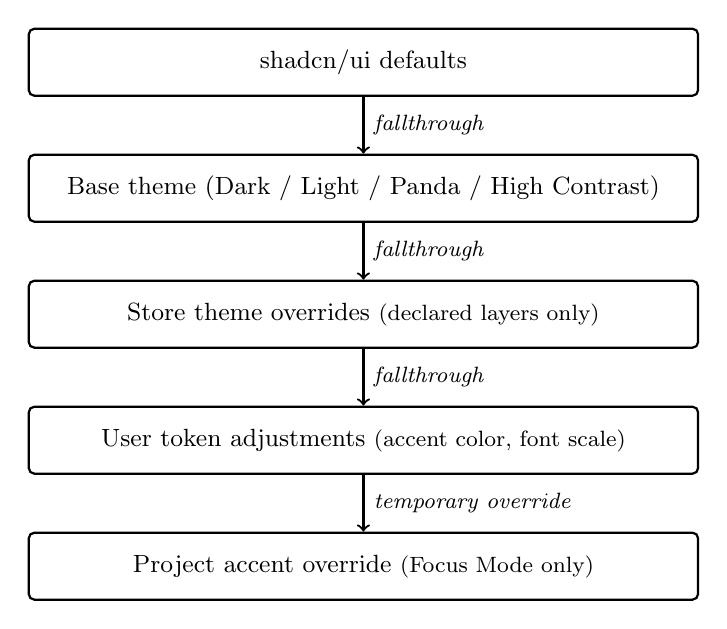
\begin{tikzpicture}[
	box/.style={
		draw, thick, rectangle, rounded corners=2pt,
		minimum width=8.5cm, minimum height=0.85cm,
		font=\small, align=center, inner sep=5pt
	},
	arr/.style={->, thick},
	lbl/.style={font=\footnotesize\itshape, anchor=west},
	]
	\def\sep{1.6}
	\node[box] (shadcn) at (0, 3*\sep)
	{shadcn/ui defaults};
	\node[box] (base)   at (0, 2*\sep)
	{Base theme (Dark / Light / Panda / High Contrast)};
	\node[box] (store)  at (0, \sep)
	{Store theme overrides \footnotesize(declared layers only)};
	\node[box] (user)   at (0, 0)
	{User token adjustments \footnotesize(accent color, font scale)};
	\node[box] (proj)   at (0, -\sep)
	{Project accent override \footnotesize(Focus Mode only)};
	\draw[arr] (shadcn) -- node[lbl, right] {fallthrough} (base);
	\draw[arr] (base)   -- node[lbl, right] {fallthrough} (store);
	\draw[arr] (store)  -- node[lbl, right] {fallthrough} (user);
	\draw[arr] (user)   -- node[lbl, right] {temporary override} (proj);
\end{tikzpicture}
\caption{Theme inheritance chain. Each layer overrides only what it declares;
everything else falls through to the layer below. The project accent override
is the outermost layer and applies only while Focus Mode is active; it is
removed when the project is deactivated, restoring the user's configured
accent. A Store theme that covers only the shell and GTK4 leaves Wine and Qt
at the base theme.}
\label{fig:theme-chain}
\end{figure}
